\documentclass{article}[a4paper]
%%%%%%%%%%%%%%%%%%%%%%%%%%%%%%%%%%%%%%%%%%%%%%%%%%%%%%%%%%%%%%%%%%
% Weimin Zhou
% 7, Nov, 2018
% upon some request, I uploaded these files for LaTeX beginners
% They could be used for Problem Set Solution typing
% startup.tex specifies all package using and title, author, abstract;
% main.tex    contains the main part of your answers.
%%%%%%%%%%%%%%%%%%%%%%%%%%%%%%%%%%%%%%%%%%%%%%%%%%%%%%%%%%%%%%%%%%
\usepackage
[
        a4paper,    % other options: a3paper, a5paper, etc
        left=1.5cm,
        right=1.5cm,
        top=2cm,
        bottom=2cm,
        % use vmargin=2cm to make vertical margins equal to 2cm.
        % us  hmargin=3cm to make horizontal margins equal to 3cm.
        % use margin=3cm to make all margins  equal to 3cm.
]
{geometry}

\usepackage[english]{babel}
\usepackage{booktabs, graphicx}   %replacing \hline
\usepackage{longtable}  % formatting tables
\usepackage{dcolumn}    %centering based on dots
\usepackage[utf8]{inputenc}
\usepackage{adjustbox}
\usepackage{blkarray}
\usepackage{color}
\usepackage[colorlinks,linkcolor=blue]{hyperref} % For cross-reference
\usepackage{amsmath,amsfonts,amssymb,amsthm} % For mathematics
\usepackage{float}    % For include graphics
\usepackage{caption,subfigure}

% For highlighting codes
\usepackage{listings}
\usepackage{xcolor} % change the color in equation 
\usepackage{textcomp}
\usepackage[framed,numbered,autolinebreaks,useliterate]{mcode}
\usepackage[section]{placeins}
\addtocounter{MaxMatrixCols}{20} % set amsmath matrix max columns  to 20 not 10


\setlength{\parindent}{4 pt}

\title{Quant Macro (Part 2)  PS2 - Solving the Krusell Smith (1998) Model with endogenous Labor Supply}

\author{Weimin Zhou}

\begin{document}
\maketitle
\begin{abstract}
	Quantitative Macroeconomics (Part 2) Problem Set 2

	I`m doing this problem set into 2 parts:

        Part 1: Question 1 for solving Aiyagari model with endogenous labor supply (the case without aggregate risk), I use two different methods: endogenous grid methods with interpolation nodes, and Sample codes from PS1 with brute-force VFI plus some modifications. 
        \medskip
        ref:

        1. \href{https://www.sas.upenn.edu/~jesusfv/companion.htm}{Companion Web Page for "Comparing Solution Methods for Dynamic Equilibrium Economies}

        2. \href{https://www.sciencedirect.com/science/article/pii/S0304393206002558}{Marcet, Albert, Francesc Obiols-Homs, and Philippe Weil. "Incomplete markets, labor supply and capital accumulation." Journal of Monetary Economics 54.8 (2007): 2621-2635.}

        Part 2: Question 2 for solving KS with endogenous labor supply (the case with aggregate risk)
\end{abstract}

\tableofcontents

\pagebreak 

%%%% Input Codes %%%%   
% <mcode.sty> required

% \lstset{numbers=left,numberstyle= \tiny}
% \lstinputlisting[firstline=6, lastline=15]{/Users/name/Desktop/FILENAME.M}

% or:

%\lstset{numbers=left,numberstyle= \tiny}
%\begin{lstlisting}[xleftmargin=2em,xrightmargin=2em,aboveskip=1em]
%clc; clear all; close all;
%\end{lstlisting}
\section{A. Model and Algorithm (without aggregate risk)}

First for {\color{red}Patial Equilibrium}, we guess a set of prices, in our simple model, we only need to guess an interest rate $r_0$ and then obtain the wage $w_0$. 
then, the household's problem in the recursive form (the Bellman equation) is:
\[
v(a,e;r_0,w_0)=max_{c,n} \{ u(c,n) + \beta \sum \pi_{e'|e} v(a',e')\}
\]
subject to the budget constraint: 
\[ 
a' = (1+r_t)a + w_t e n - c
\]

And for {\color{red} General Equilibrium}, we loop for above stationary equilibrium, computing the error between the obtain prices and the initial guess prices, till the convergence of market clearing.



%%%%%%%%%%%%%%%%%%%%%%%%%%%%%%%%%%%%%%%%%%%%%%%%%%%%%%%%%%%%
\section{A. Solution of the stochastic model with endogenous labor supply (without aggregate risk)}
Abstract from aggregate risk and fix  the TFP $z_t = \bar{z}$ for all $t$.

% Please add the following required packages to your document preamble:
% \usepackage{booktabs}
\begin{table}[]
\begin{tabular}{@{}cccc@{}}
\toprule
file name                 & Content                                                                                                                                                           & Associated files          & Comments                                                                                               \\ \midrule
sample\_divisible\_labor.m & \begin{tabular}[c]{@{}c@{}}Compute the stationary general equilibrium of \\ Aiyagari with endogenous elastic labor supply\end{tabular}                            & stationary\_equilibrium.m & \begin{tabular}[c]{@{}c@{}}using interpolation for obtaining\\ the choice beyond the grid\end{tabular} \\
Q1main.m                  & \begin{tabular}[c]{@{}c@{}}The main methods I'm using for Question-1\\ (both Partial Equilibrium and GE included)\end{tabular}                                    & general\_equilibrium.m    & \begin{tabular}[c]{@{}c@{}}generating separate grids also for \\ labor.\end{tabular}                   \\
Q1alter.m                 & \begin{tabular}[c]{@{}c@{}}Compute Question-1 using "fsolve" for consumption and then obtain labor \\ for every grid points of assets\\ , and do VFI\end{tabular} & -                         & Time-consuming                                                                                        
\end{tabular}
\end{table}


\subsection{Household problem}
%%%%%%%%%%%%%%%%%%%%%%%%%
\subsubsection{Write down the problem of the household in a recursive form and find the optimal intratemporal and intertemporal conditions.}

The household problem solves:

\begin{align} \label{hhproblem}
\begin{split}
v(k,\epsilon; \Gamma ,z) &= \max_{c,k'} \{ u(c) - v(h) + \beta E [v(k',\epsilon'; \Gamma' ,z')| z, \epsilon]\} \\
\text{subject to} \\
& c + a' = r(z,\mu)a + w(z,\mu)h \epsilon + (1-\delta)a \\
& \mu' = H(\mu) \\
& a' \geq -B \\
\text{where:} \\
&u(c) - v(h) = \frac{c^{1-\sigma} - 1}{1 - \sigma} - \Gamma \frac{h^{1+1/\nu}}{1+1/\nu} \\
\end{split}
\end{align}

{\color{red} In Question 1, there's no aggregate risk, and we only guess the prices, but not use firms conditions for market clearing}

Note: to accelerate convergence. Some papers start iterating on a small grid. Then, after convergence, add more points to the grid, and recompute the Bellman operator using the previously found value function as aninitial guess (with linear interpolation to fill the unknown values in the new gridpoints).



Then, the optimal conditions characterize the household's choice are the following:

\begin{align}
v'(h_t) &= u'(c_t)w_t \epsilon_t \text{, intratemporal condition }\\
u'(c_t) &= \beta E_t [u'(c_{t+1})(1+r_t)] + \mu_t  \text{, intertemporal condition }\\
\mu_t (a_{t+1} + B) &= 0 \text{ , } \mu_t \geq 0 \\
a_{t+1} &= (1+r_t)a_t + h_t \epsilon_t w_t - c_t 
\end{align}

\subsubsection{Use the intratemporal condition and the budget constraint to write the problem of the household in terms of a single decision variable}

First, we use the inversion function of the marginal disutility of labor from the intratemporal optimality condition to derive: 
\[ H(c_t, \epsilon_t) = (v')^{-1}(u'(c_t)\epsilon_t w_t)\]
and in our special separable CRRA utility case, this has analytical solution: 
\[ H(c,y) = (\frac{c^{-\sigma \epsilon w}}{\Gamma})^{-1/\gamma} \]

Then, solve consumption by Budget Constraint, use above information:
\[ c = (1+r)a + w H(c,y)e  - a'\] 
and denote the solution of consumption as $C(a',e)$ given grid of $a'$ and $e$. 

Then, we simply rewrite the Bellman Equation \ref{hhproblem} as: 
\begin{align}
v(a,e; \Gamma ,z) &= \max_{a'} \{ u\{(1+r)a + H((C(a',e)),y)\}  - v(H(C(a',e),y)) \\
& + \beta E [v(k',\epsilon'; \Gamma' ,z')| z, \epsilon]]
\end{align} 

\pagebreak
%%%%%%%%%%%%%%%%%%%%%%%%%%%%%%%%%%%%%%%%%%%%%%%%%%
\subsubsection{For a given value of wages and the interest rate, write the code to solve for the policy function of a`}

{\color{red} Use the transition matrix from PS1, implied by good times $\pi_{gge'e}$ and bad times $\pi_{bbe'e}$ respectively.}

See code,  {\color{red} Q1.m} and alternative method for sovling this problems are listed in \textbf{Q1alter.m, Q1alter1.m}.


\begin{figure}[htbp]
\centering
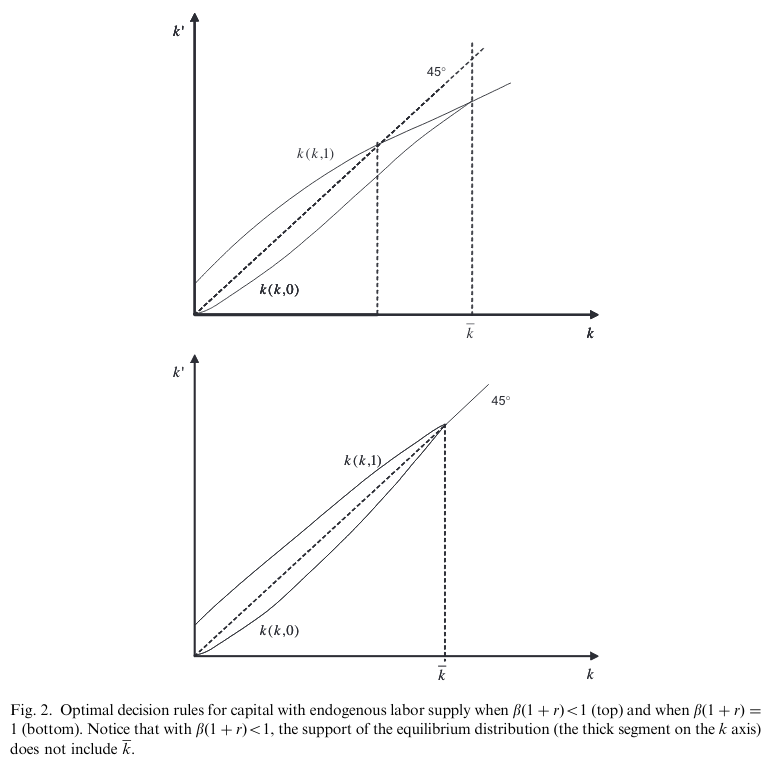
\includegraphics[width=\textwidth]{img/sample.png}
\caption{$a'(e,a)$ in Marcet, Obiols-Homs, Weil(2007) Figure 2 for different cases}
\end{figure}

A standard results related to this problem should have similar decision rule as above Figures by Marcet, Obiols-Homs, Weil(2007), where they use Newton methods for solving first order and feasibility conditions, and finds decision rules for capital and leisure by approximating the derivative of the value function with piece-wise linear functions on agrid of points for state variables.


\subsubsection*{part (a + b) compare policy function for two transition matrix}

Unlike above figure, since I'm not using any approximation methods for below figures, and I didn't check the bonded above limit for assets, hence (the drawback of discretization methods now is much more clear: the grids I choose will interfere much on the figure). 

\begin{figure}[htbp]
\centering
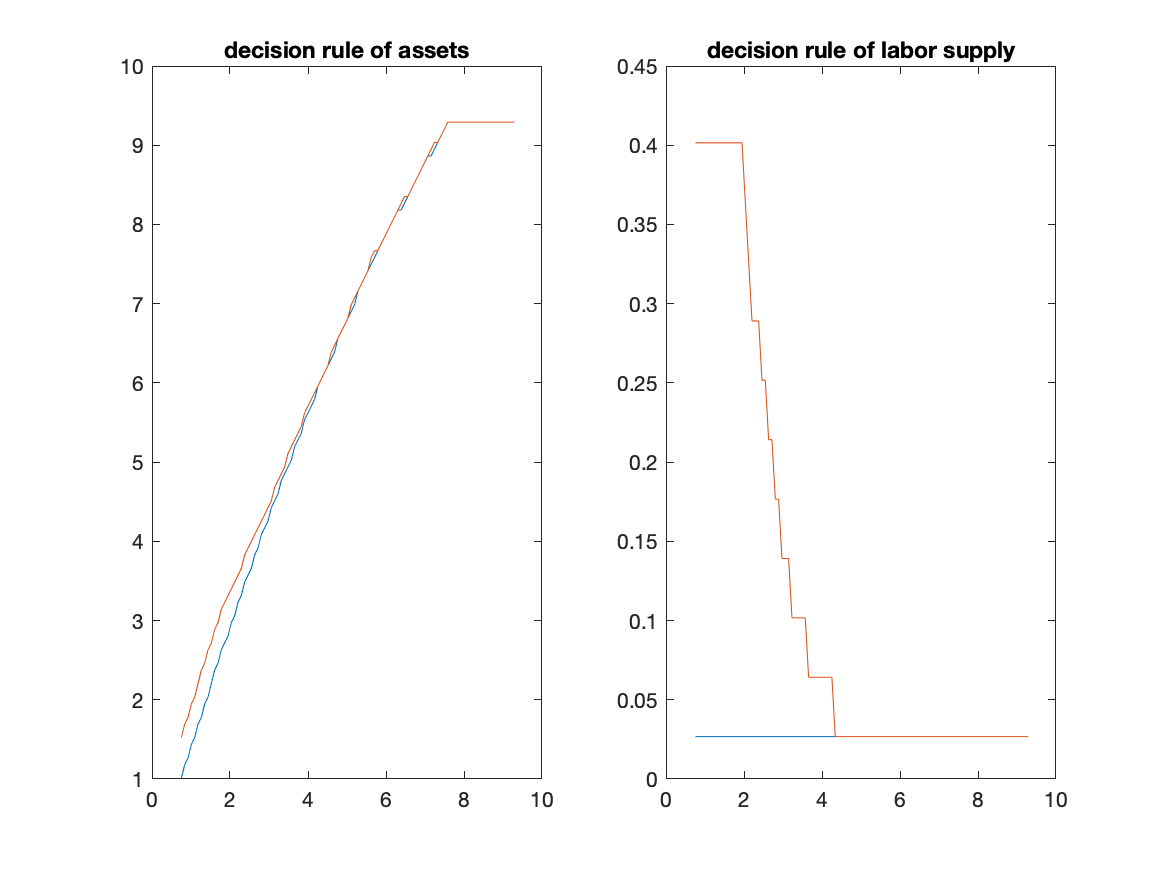
\includegraphics[width=\textwidth]{img/Q1.png}
\caption{$a'(e,a)$ and $n(e,a)$ in good transition matrix}
\end{figure}

\begin{figure}[htbp]
\centering
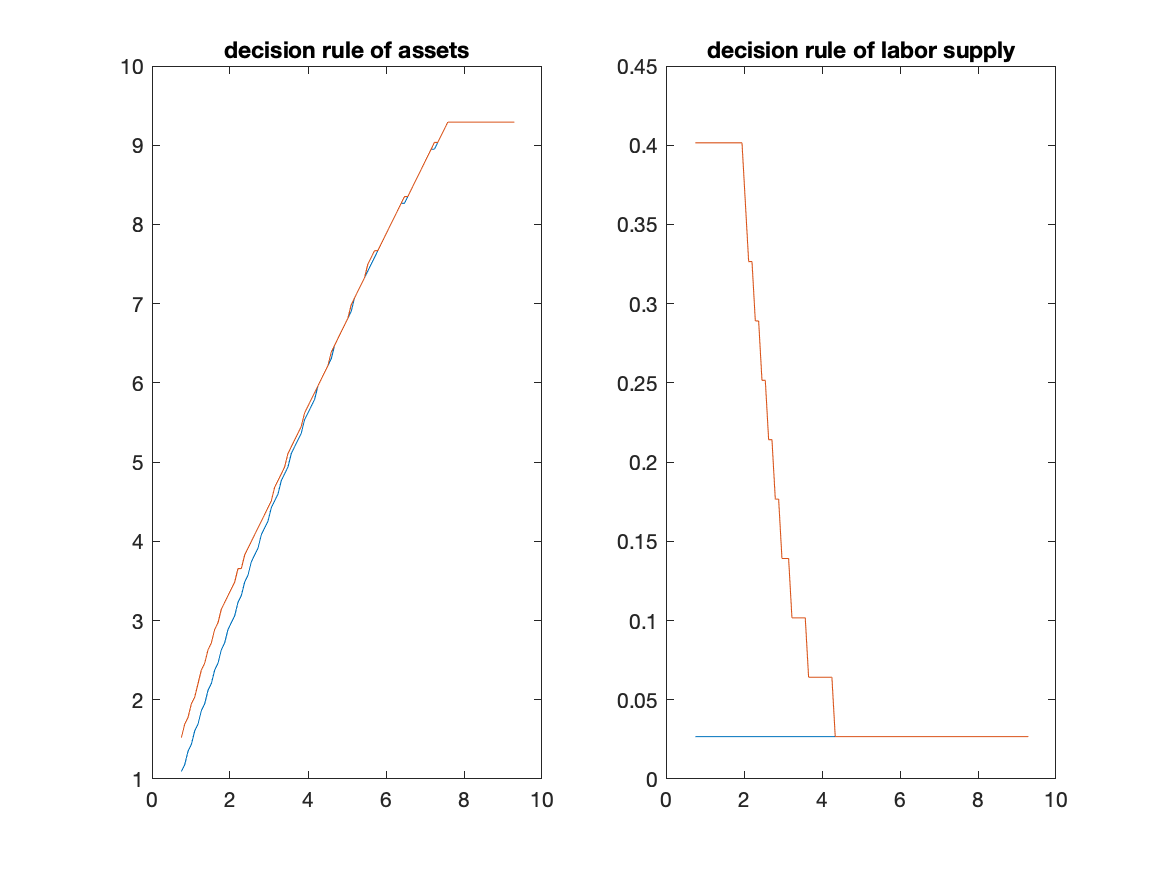
\includegraphics[width=\textwidth]{img/Q1-bad.png}
\caption{$a'(e,a)$ and $n(e,a)$ in bad transition matrix}
\end{figure}

Since by looking at two transition matrix, there's no too big difference, hence the value and evolution of decision rules are similar only for bad transition matrix, the assets decisions rule are accumulated lower than the one in good transition matrix. 

%%%%%%%%%%%%%%%%%%%%%%%%%
\subsection{General Equilibrium}
\subsubsection{Equilibrium conditions in the capital, labor and goods markets}

the equilibrium conditions are:

goods market clear:
\[ f(K_t,N_t) + (1-\delta)K = C + K'\]

capital market clear:
\begin{align}
K = \int_{a_{min}}^{a_{max}} \sum_{y\in Y} g(a,y) \Gamma (a,y) d a
\end{align}

labor market clear is also the sum upo of individuals' supplys equal to Aggregate Labor demand from firms, and by Warlas' law, no need to have anymore once goods market and capital market clear.


\subsection{Solve for the equilibrium}

The method we are using are very sentitive to our initial guess value, whereas many of us are randomly guessing, in my results, since the staionary distribution is very sensitive to the interst rate. I make use of the theoretical result that the stationary rate is slightly 
 below 1/beta-1. Based on this, the genreal equilibrium is converged to $r = 0.0409$ for my set-up on $z_H = 1.6$, and  $r = 0.0404$ for $z_L = 0.8$. 

 Simulation results:

for z\_H = 1.6:\\
r1 = 0.0525\\
 r2 = 0.0466, residual = -0.1132\\
 r3 = 0.0436, residual = -0.0650 done..\\
 ...\\
 rn = 0.0409, residual = -0.0098\\
 for z\_L = 0.8:\\
 r1 = 0.0525\\
 r2 = 0.0693, residual = -0.0620\\
 r3 = 0.0469, residual = -0.0490\\
 ...\\
 rn = 0.0404, residual = -0.0085\\

\subsubsection{Calibrate}

Based on Luis's advice, I keep $\gamma=3/2$ in my model not change, with a $\frac{N_{zl}+ N_{zh}}{2}=\bar{N}=0.9731$, I calibrate a $\Gamma = 0.5600$.

This part is associated with {\color{red} \textbf{Q1main.m} line [388-500]};

\pagebreak

%%%%%%%%%%%%%%%%%%%%%%%%%%%%%%%%%%%%%%%%%%%%%%%%%%
\section{B. Model and Algorithm (with aggregate risk)}
Krusell\&Smith(1998) develop a computational algorithm to approximate the equilibrium. The main challenge is to compute the law of motion for the aggregate states.

Now the agent solves the following problem: 
\begin{align}
V(\omega,\epsilon,\bar{k},z) = \max u(\omega + n \epsilon * F_2 (\bar{k},H^n (\bar{k},z),z) + k - k', n)+\\
\beta E [V(k'(1-\delta + F_1 (H^k (\bar{k},z),H^n ((H^k (\bar{k},z),z'),z')),\epsilon',H^k (\bar{k},z)| z,\epsilon] \\
\text{s.t. } \bar{k'} = H^k(\bar{k},z) = a^z_{0} + a^z_{1} \bar{k} \text{ , and } \bar{n}=H^n (\bar{k},z)=c^z_0 + c^z_1 \bar{k}\\ 
\end{align}
\subsection*{Algorithm}
Since  there  is  aggregate  uncertainty  but  no  aggregation,  we  have  to  use  a  Krusell-Smith  algorithm.  Note, however, that since labor is endogenous, and the labor supply is not fixed, capital is not a sufficient forecast for all future prices, next period.  In other words, the agent has to forecast $r$ and $w$ in order to optimize.  In a setting with fixed labor supply, a forecast of $K$ gives us a forecast of $K/H$, which in turn allows the agent to forecast marginal productivities and both prices.  Now, $H$ is no longer fixed hence two forecasts are required.  Assume that agents use the following forecasting rules: 
\begin{align}
log K' = b^0_z + b^1_z log K \\
log H  = d^0_z + d^1_z log K \text{ or: } log H' = d^0_Z + d^1_z log H, 
\end{align}

And then the algorithm goes as follows:
\begin{enumerate}
\item Guess coefficients for the perceive laws of motion $b^0_z, b^1_z, d^0_z, d^1_z$ where, $z\in{z_g,z_b}$ and Initial decision rules $g_a (e,a,z,K;H)$ and $g_h (e,a,z,K;H)$
\item Solve  the  household  problem  and  obtain  the  decision  rules $(c,a',h)(a,\epsilon;Z,\lambda)$ with the foecasts of $(r',w',\pi')$ are required. For the first two, our laws of motion are enough. Goods market clearing also implies that: 
\[ Y + (1-\delta)K = C + K' \]
\item Simulate the economy for N individuals and T periods. Draw first a sequence of aggregate shocks ${z_t}_{t=1}^T$. Then, draw individual productivity shocks ${\epsilon_{it}}_{t=1,i=1}^{T,N}$ (potentially onditional on the path of the aggregateshocks, if there were correlation).  Given initial conditions for each agent ${a_0i}^N_{i=1}$, compute the path of policies ${(a_{it}, h_{it})}_{i=1,t=1}^{N,T}$. For each period, compute the average capital stock and labor supply:
\begin{align}
\hat{K_t} = \frac{1}{N} \sum_{i=1}^N a_{it} \\
\hat{H_t} = \frac{1}{N} \sum_{i=1}^N \epsilon_{it} h_{it}
\end{align}
\item Note that in this model, we need to clear three different markets (capital, labor and the government budget constraint) every period (the fourth, goods, clears by Walras’ Law).  In order to avoid numerical instability, we should make sure that all markets clear at each $t$.  Therefore, an additional inner loop is required:  if $\hat{H_t}$ does not coincide with the forecast, update $w_t$ until the labor market clears.  At the same time, since $H$ is changing, so is $Y$, need to update goods market clearing 

\item Discard the first S periods in order to avoid dependence on initial conditions. Using the remaning sequences, regress the following:
\begin{align}
log \hat{K}_{t+1} = b^0_z + b^1_z log \hat{K}_{t} \\
log \hat{H}_{t+1} = d^0_z + d^1_z log \hat{K}_{t} 
\end{align}

and estimate the parameters. 

\item For a given tolerance level $\eta$, check the criterion for converenges on above parameters. If yes, then stop, otherwise replace the parameters and return to STEP 2. 

\item  Recall that this equilibrium is approximate:  we still need to verify how good this approximation is to thefully rational-expectation equilibrium.  For this purpose, compute a measure to the fit of the regression,for example by using $R^2$. 
\end{enumerate}



\section{B. Solution and Simulation of the stochastic model with endogenous labor supply (with aggregate risk)}

Even though there are no contracts that can be explicitly traded to insure unemployment risk, in this economy self-insurance through borrowing/saving and though divisible labor supply provides good hedging against wage risk. So, we are somewhat close to the complete markets case in Krusell and Smith (1998). 

\subsection{Using 'fsolve' for every generating grids}
This methods is super slow, so I commented them on my codes, but for a more complete solution, here I attached the Algorithm I use:

1. Define first-step decision rulesfor assets and hours worked $g_a (e,a,z,K;H)$ and $g_h (e,a,z,K;H)$, a a function of aggregate labor input H as well

Define Perceived Law of Motion: 
\begin{align}
log \hat{K}_{t+1} = b^0_z + b^1_z log \hat{K}_{t} \\
log \hat{H}_{t+1} = d^0_z + d^1_z log \hat{K}_{t} 
\end{align}

2. Guess initial decision rules and aggregate laws of motion

3. At every point on the grid solve for $(h,a)$ using the Equilibrium condition:
\begin{align}
&u_c (R(z,K,H)a + w(z,K,H)eh^* - a^*) = \beta \cdot\\
&  \{ R(z',K',H')\cdot u_c(r(z',K',H')a + w(z',K',H'))a^* + \\
&w(z',K',H')e' g_h (e',a^*,z',K';H') \\
&- g_a (e',a^*,z',K';H')\} \pi_{z'ze'e} \\
&\text{ and the intratemporal condition: } \\
&v_h (h^*) = w(z,K,H)e \cdot u_c (R(z,K,H)a + w(z,K,H)e - a^*)
\end{align}

4. Once these first-step decision rules are obtained from this system  of equations, use the decision rules to simulate an artificial panel,but at every date t one must solve for $H^*_t$ that satisfies the laborm arket clearing condition at date t:
\[ \sum g_h (e,a,z_t,K_t,H^*_t) = F_H (\frac{w(z_t,K_t,H^*_t)}{z_t},K_t)^{-1}\]

5. This time series ${z_t,H^*_t,K_t}$ is used to update the guess of the aggregate laws of motion.

6. Once converged is achieved, we can solve for the second-step (and final) decision rules only as a function of K

\pagebreak

\subsection{Updated Figures}

\begin{figure}[htbp]
\centering
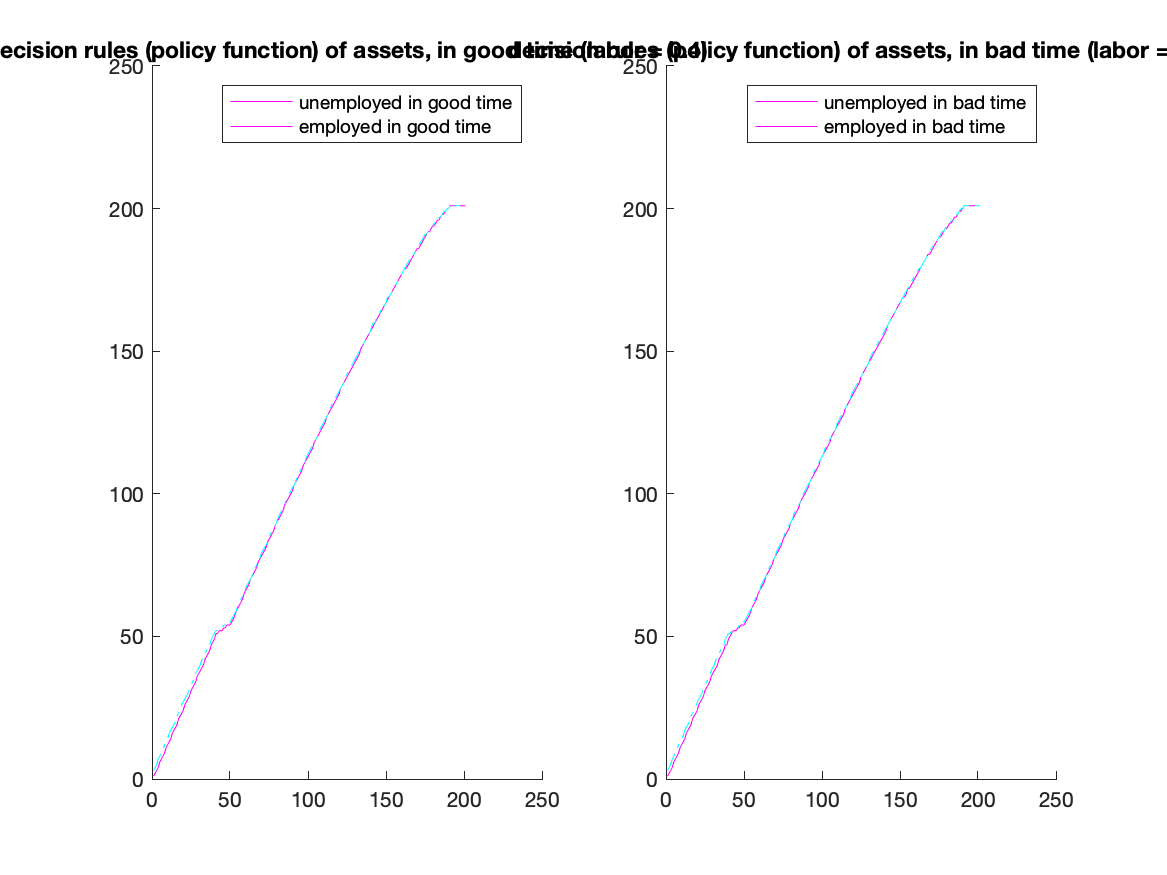
\includegraphics[width=\textwidth]{img/Q2_1_plot.png}
\caption{$a'(e,a)$  given different idiosyncratic risks at $h=0.4$}
\end{figure}


 




\pagebreak

\end{document}